\documentclass{article}%
\usepackage[T1]{fontenc}%
\usepackage[utf8]{inputenc}%
\usepackage{lmodern}%
\usepackage{textcomp}%
\usepackage{lastpage}%
\usepackage[head=40pt,margin=0.5in,bottom=0.6in]{geometry}%
\usepackage{graphicx}%
%
\title{\textbf{Audiencia de funcionarios del Sebin relacionados al caso Albán fue diferida}}%
\author{El Nacional Web}%
\date{23/11/2018}%
%
\begin{document}%
\normalsize%
\maketitle%
\textbf{URL: }%
http://www.el{-}nacional.com/noticias/politica/audiencia{-}funcionarios{-}del{-}sebin{-}relacionados{-}caso{-}alban{-}fue{-}diferida\_260906\newline%
%
\textbf{Periodico: }%
EN, %
ID: %
260906, %
Seccion: %
Política\newline%
%
\textbf{Palabras Claves: }%
Política, Sebin\newline%
%
\textbf{Derecho: }%
1.1, %
Otros Derechos: %
1.10, %
Sub Derechos: %
1.1.1.3, 1.10.1\newline%
%
\textbf{EP: }%
NO\newline%
\newline%
%
\textbf{\textit{Los uniformados son acusados de "quebrantamiento del deber de custodia"~}}%
\newline%
\newline%
%
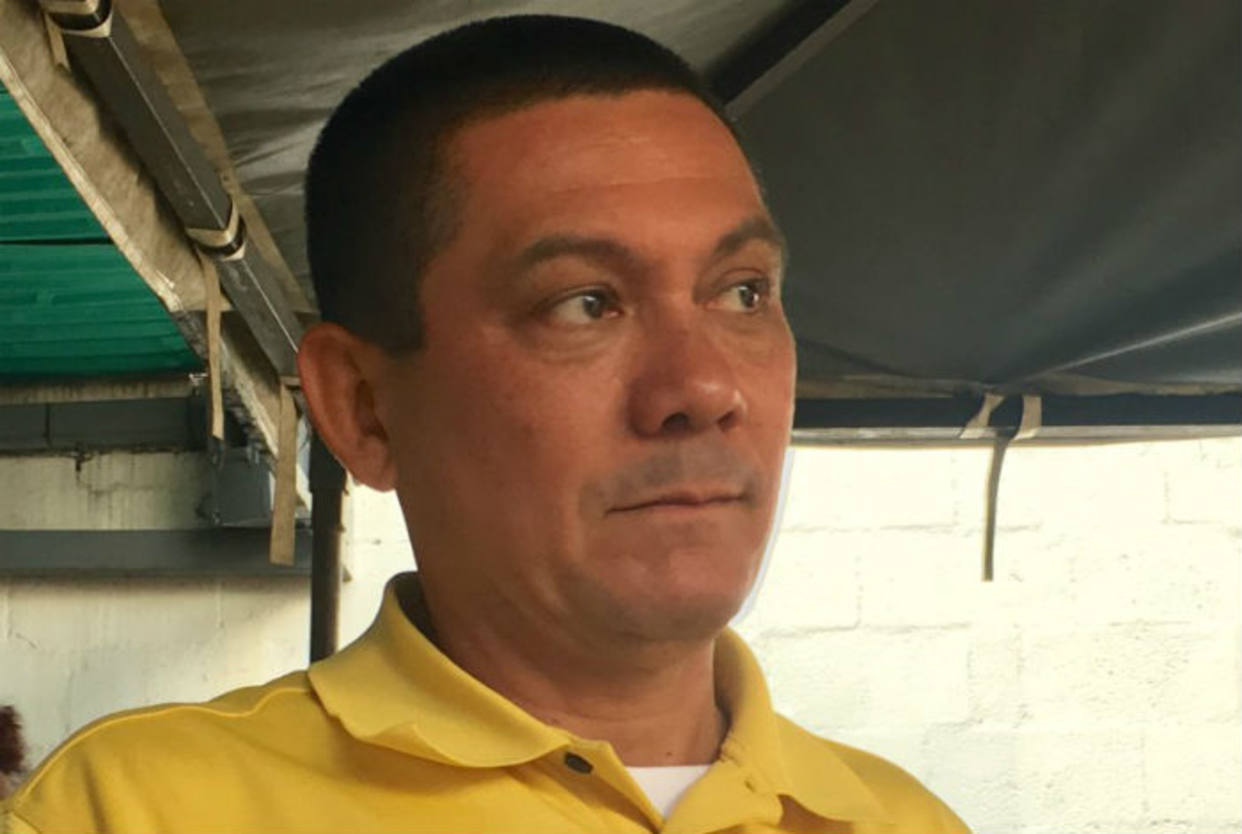
\includegraphics[width=300px]{103.jpg}%
\newline%
%
La audiencia de presentación de los funcionarios del Servicio Bolivariano de Inteligencia Nacional que serían imputados por~la muerte del concejal Fernando Albán, no se realizó este viernes debido a que los acusados y los miembros de la Fiscalía del Ministerio Público no llegaron al lugar a la hora pautada.%
\newline%
%
En la audiencia, a cargo del juez Fredy Pérez, se imputaría a los funcionarios por “quebrantamiento del deber de custodia”.%
\newline%
%
Cuando los abogados solicitaron información sobre el hecho, María Gabriela la Rosa, secretaria del Tribunal, informó que “Fernando Albán no aparece como víctima en ese proceso” y se negó a recibir el poder que exhibieron los abogados para acreditar su legitimación y actuar en la audiencia.%
\newline%
%
Ramón Alfredo Aguilar, Enrique Serra y Susnaikyl Corniel, abogados de la familia Albán, pueden actuar y solicitar la aplicación del Protocolo de Minessota, Protocolo de Estambul y del Pacto Internacional de los Derechos Civiles debido a que consideran que la muerte del concejal fue “potencialmente ilícita”.%
\newline%
%
Con información de nota de prensa%
\newline%
%
\end{document}